
\paragraph{GET /:lang/user/:userId/question}
\begin{itemize}
\item \textbf{Successo}\\
Questo scenario rappresenta il successo di una richiesta che ritorna tutte le domande create da un utente che impone, come vincolo per poter essere effettuata, che l'utente sia autenticato al sistema; quindi prima di tale operazione deve venire fatta una richiesta di controllo di sessione mediante l'apposita \textit{REST\ped{G}}. In questo caso il modulo \texttt{QuestionController} invia \texttt{next()} per indicare il successo dell'operazione.

\begin{figure}[ht]
	\centering
	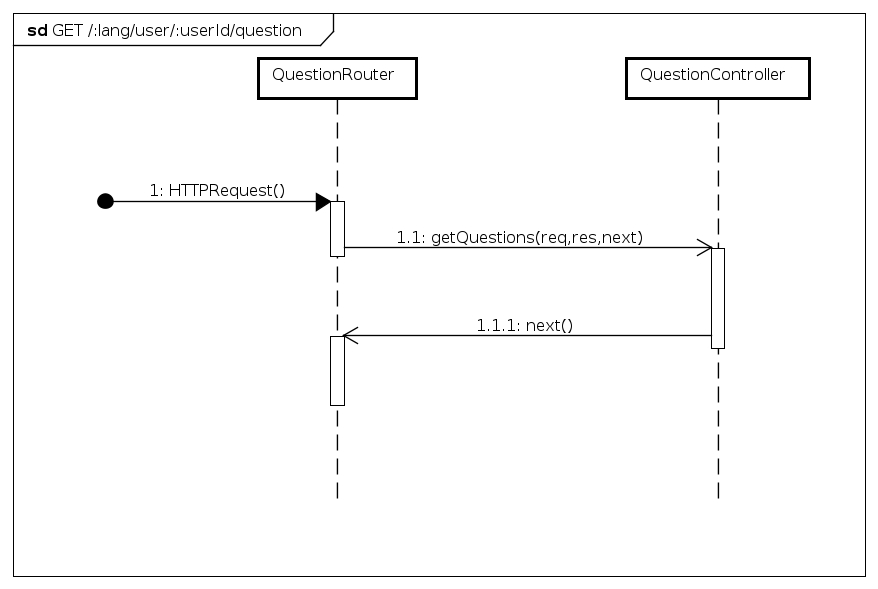
\includegraphics[scale=0.45]{UML/DiagrammiDiSequenza/Back-end/GET__lang_user__userId_question_success.png}
	\caption{Successo: GET /:lang/user/:userId/question}
\end{figure}
\FloatBarrier

\item \textbf{Fallimento}\\
Questo scenario rappresenta il fallimento di una richiesta che ritorna tutte le domande create da un utente che impone, come vincolo per poter essere effettuata, che l'utente sia autenticato al sistema; quindi prima di tale operazione deve venire fatta una richiesta di controllo di sessione mediante l'apposita \textit{REST\ped{G}}. In questo caso il modulo \texttt{QuestionController} invia \texttt{next(error)} per indicare il fallimento di tale vincolo al router il quale avrà compito di reinstradarlo (indirizzandolo verso \texttt{ErrorHandler}).

\begin{figure}[ht]
	\centering
	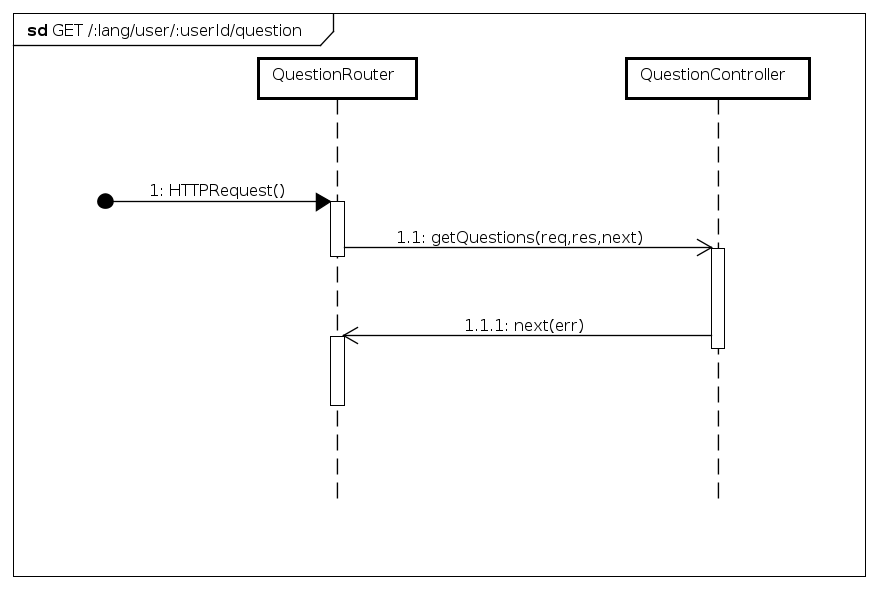
\includegraphics[scale=0.45]{UML/DiagrammiDiSequenza/Back-end/GET__lang_user__userId_question_failure.png}
	\caption{Fallimento: GET /:lang/user/:userId/question}
\end{figure}
\FloatBarrier

\end{itemize}






\paragraph{GET /:lang/user/:userId/question/:questionId}
\begin{itemize}
\item \textbf{Successo}\\
Questo scenario rappresenta il successo di una richiesta che ritorna una domanda creata da un utente che impone, come vincolo per poter essere effettuata, che l'utente sia autenticato al sistema; quindi prima di tale operazione deve venire fatta una richiesta di controllo di sessione mediante l'apposita \textit{REST\ped{G}}. In questo caso il modulo \texttt{QuestionController} invia \texttt{next()} per indicare il successo dell'operazione.


\begin{figure}[ht]
	\centering
	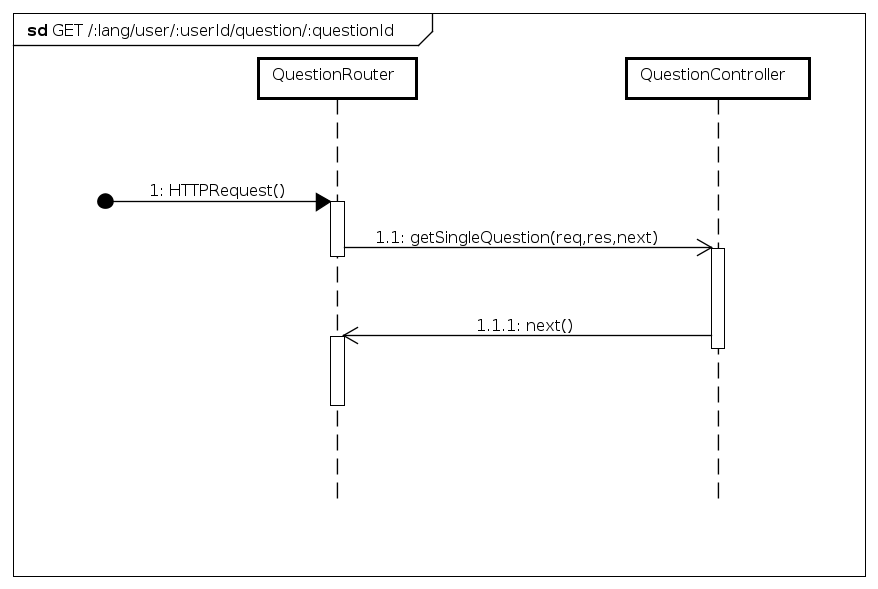
\includegraphics[scale=0.45]{UML/DiagrammiDiSequenza/Back-end/GET__lang_user__userId_question__questionId_success.png}
	\caption{Successo: GET /:lang/user/:userId/question/:questionId}
\end{figure}
\FloatBarrier

\item \textbf{Fallimento}\\
Questo scenario rappresenta il fallimento di una richiesta che ritorna una domanda creata da un utente che impone, come vincolo per poter essere effettuata, che l'utente sia autenticato al sistema; quindi prima di tale operazione deve venire fatta una richiesta di controllo di sessione mediante l'apposita \textit{REST\ped{G}}. In questo caso il modulo \texttt{QuestionController} invia \texttt{next(error)} per indicare il fallimento di tale vincolo al router il quale avrà compito di reinstradarlo (indirizzandolo verso \texttt{ErrorHandler}).

\begin{figure}[ht]
	\centering
	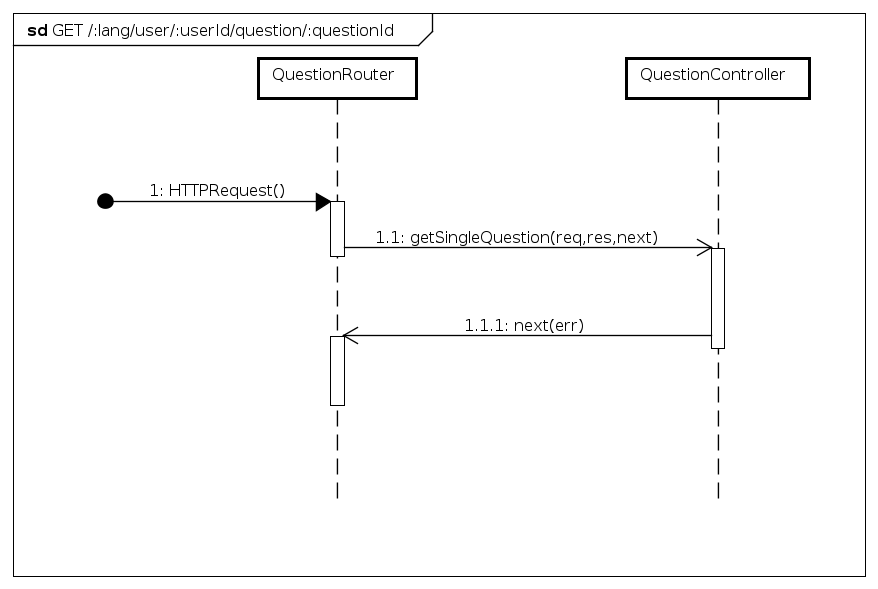
\includegraphics[scale=0.45]{UML/DiagrammiDiSequenza/Back-end/GET__lang_user__userId_question__questionId_failure.png}
	\caption{Fallimento: GET /:lang/user/:userId/question/:questionId}
\end{figure}
\FloatBarrier

\end{itemize}






\paragraph{POST /:lang/user/:userId/question}
\begin{itemize}
\item \textbf{Successo}\\
Questo scenario rappresenta il successo di una richiesta che inserisce una nuova domanda creata da un utente all'interno del sistema che impone, come vincolo per poter essere effettuata, che l'utente sia autenticato al sistema; quindi prima di tale operazione deve venire fatta una richiesta di controllo di sessione mediante l'apposita \textit{REST\ped{G}}. In questo caso il modulo \texttt{QuestionController} invia \texttt{next()} per indicare il successo dell'operazione.


\begin{figure}[ht]
	\centering
	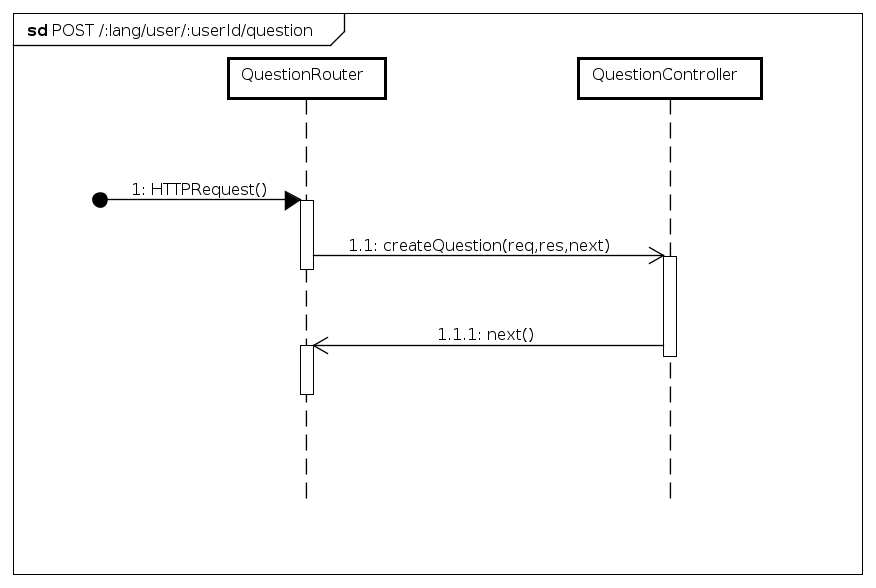
\includegraphics[scale=0.45]{UML/DiagrammiDiSequenza/Back-end/POST__lang_user__userId_question_success.png}
	\caption{Successo: POST /:lang/user/:userId/question}
\end{figure}
\FloatBarrier

\item \textbf{Fallimento}\\
Questo scenario rappresenta il fallimento di una richiesta che inserisce una nuova domanda creata da un utente all'interno del sistema che impone, come vincolo per poter essere effettuata, che l'utente sia autenticato al sistema; quindi prima di tale operazione deve venire fatta una richiesta di controllo di sessione mediante l'apposita \textit{REST\ped{G}}. In questo caso il modulo \texttt{QuestionController} invia \texttt{next(error)} per indicare il fallimento di tale vincolo al router il quale avrà compito di reinstradarlo (indirizzandolo verso \texttt{ErrorHandler}).

\begin{figure}[ht]
	\centering
	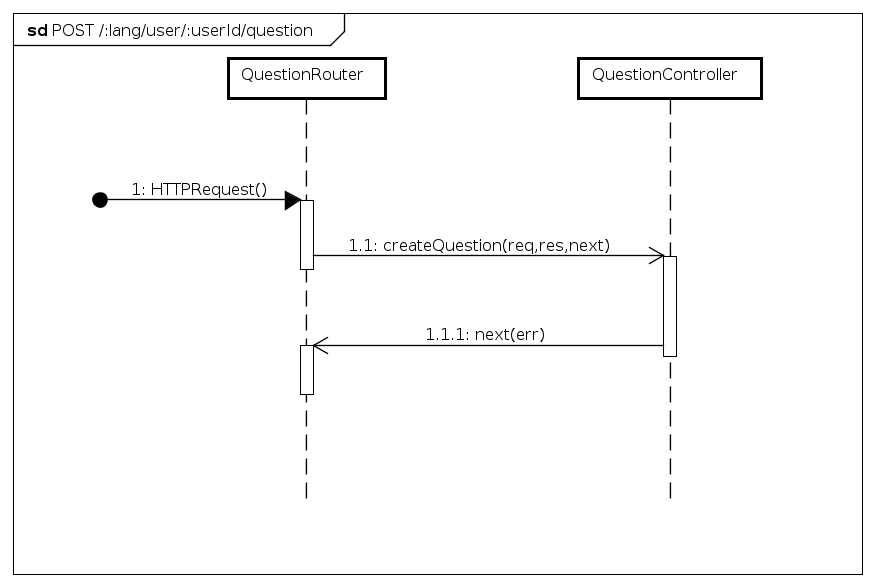
\includegraphics[scale=0.45]{UML/DiagrammiDiSequenza/Back-end/POST__lang_user__userId_question_failure.png}
	\caption{Fallimento: POST /:lang/user/:userId/question}
\end{figure}
\FloatBarrier

\end{itemize}
